%*******************************************************************************
% Master TeX file for 6x9 books
% Copyright A K Peters, Ltd.
%
% This is the main TeX file that is to be compiled.
%*******************************************************************************
\documentclass{book}

%*******************************************************************************
% Layout
%
% This defines the size of the page, etc. DO NOT EDIT.
%*******************************************************************************
\usepackage{geometry}

\geometry{
  paperwidth=6in,
  paperheight=9in,
  width=27pc,
  height=45pc, % textheight + head + headsep = 45pc
  headsep=12pt,
  foot=24pt,
  inner=0.9375in, % 15/16 in. gutter margin
  top=0.625in, % head margin
  includehead
}

% draws crop marks
\usepackage[cam,center,letter,noinfo]{crop}

\newcommand*\altcropulc{%
\begin{picture}(0,0)
 \unitlength = 1pt
 \thinlines
 \put(-30,0){\circle{10}}
 \put(-30,-5){\line(0,1){10}}
 \put(-35,0){\line(1,0){21}}
 \put(0,30){\circle{10}}
 \put(-5,30){\line(1,0){10}}
 \put(0,35){\line(0,-1){21}}
 \end{picture}
}

\newcommand*\altcropurc{%
 \begin{picture}(0,0)
 \unitlength = 1pt
 \thinlines
 \put(30,0){\circle{10}}
 \put(30,-5){\line(0,1){10}}
 \put(35,0){\line(-1,0){21}}
 \put(0,30){\circle{10}}
 \put(-5,30){\line(1,0){10}}
 \put(0,35){\line(0,-1){21}}
 \end{picture}%
}

\newcommand*\altcropllc{%
 \begin{picture}(0,0)
 \unitlength = 1pt
 \thinlines
 \put(-30,0){\circle{10}}
 \put(-30,-5){\line(0,1){10}}
 \put(-35,0){\line(1,0){21}}
 \put(0,-30){\circle{10}}
 \put(-5,-30){\line(1,0){10}}
 \put(0,-35){\line(0,1){21}}
 \end{picture}%
}

\newcommand*\altcroplrc{%
 \begin{picture}(0,0)
 \unitlength = 1pt
 \thinlines
 \put(30,0){\circle{10}}
 \put(30,-5){\line(0,1){10}}
 \put(35,0){\line(-1,0){21}}
 \put(0,-30){\circle{10}}
 \put(-5,-30){\line(1,0){10}}
 \put(0,-35){\line(0,1){21}}
 \end{picture}%
 }

\cropdef\altcropulc\altcropurc\altcropllc\altcroplrc{altcrop}

\crop[altcrop]

%*******************************************************************************
% Style file
%*******************************************************************************
\usepackage{akpbook}

%*******************************************************************************
% Packages
%
% Here you can add your own packages, if necessary, that are not covered by akpbook.sty
%*******************************************************************************
%---BEGIN AUTHOR EDIT---

\usepackage{subfig}
\usepackage{multirow}

%---END AUTHOR EDIT---

%*******************************************************************************
% Declarations
%
% Any custom commands, aliases, or other declarations should be added to
% a separate TeX file, called [your last name]Macros.tex (e.g., SmithMacros.tex)
%*******************************************************************************
%---BEGIN AUTHOR EDIT---

%\include{[your last name]Macros}

%---END AUTHOR EDIT---

%*******************************************************************************
% Figure folders
%
%   Save you figures in a subfolder of the folder that contains this TeX file,
%   called Figures.
%
%   Uncomment the line below if your article contains figures.
%
%   Figures can then be included in the document using:
%
%   \includegraphics[width=\textwidth](FigFileName.eps}
%
%   or similar command.
%*******************************************************************************
\graphicspath{{Figures/}} % you may uncomment this line if needed

%*******************************************************************************
% Book
%*******************************************************************************
\makeindex
\begin{document}

\mainmatter
 \renewcommand{\chaptermark}[1]{\markboth{\thechapter. #1}{}}
 \renewcommand{\sectionmark}[1]{\markright{\thesection. #1}}

%*******************************************************************************
% Your Chapter
%
% The main body of your article should be a file called [your last name].tex.
%
% For the sake of this template, we provide a file called Smith.tex. You should
% edit the line below to match the name of your file, i.e., your last name.
%*******************************************************************************

%---BEGIN AUTHOR EDIT---
\chapter{Parallax-Corrected Cached Shadow Maps}{Pavlo Turchyn}
 \label{Turchyn-chapter}

\section{Introduction}

Rendering shadows over large viewing distances often requires 
processing a large number of shadow-casting objects. Many game
engines, which are using shadow maps for long-range shadow rendering,
opt for some caching schemes that allow distributing the costs of shadow 
map rendering over several frames, thus exploiting frame-to-frame
coherency and rendering only a subset of shadow casters per frame,
e.g. \cite{CrytekRyse}\cite{CSMScrolling}. Some game engines cache occlusion data 
derived from shadow maps rather than keeping plain shadow maps, e.g. 
\cite{ShadowsInGames}\cite{WitcherTerrain}. 

\begin{figure}[h]
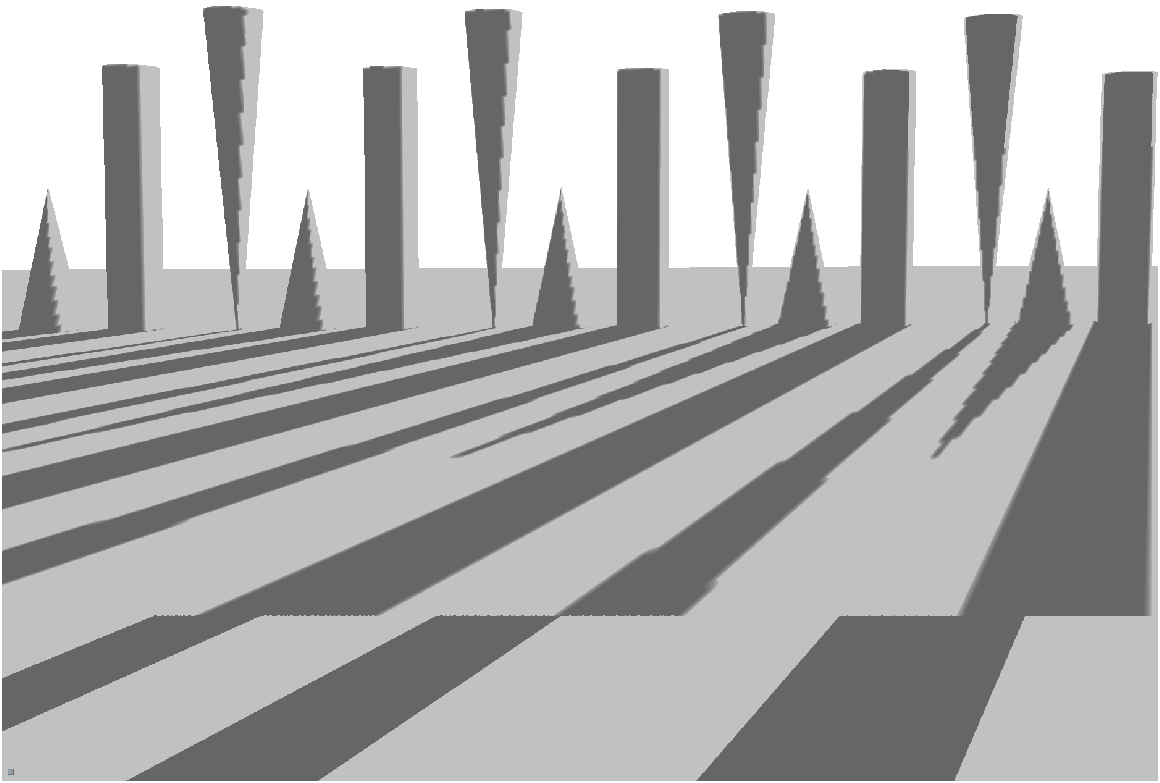
\includegraphics[width=0.48\textwidth]{pcsm_1a.pdf}\label{Teaser:a}\hfill
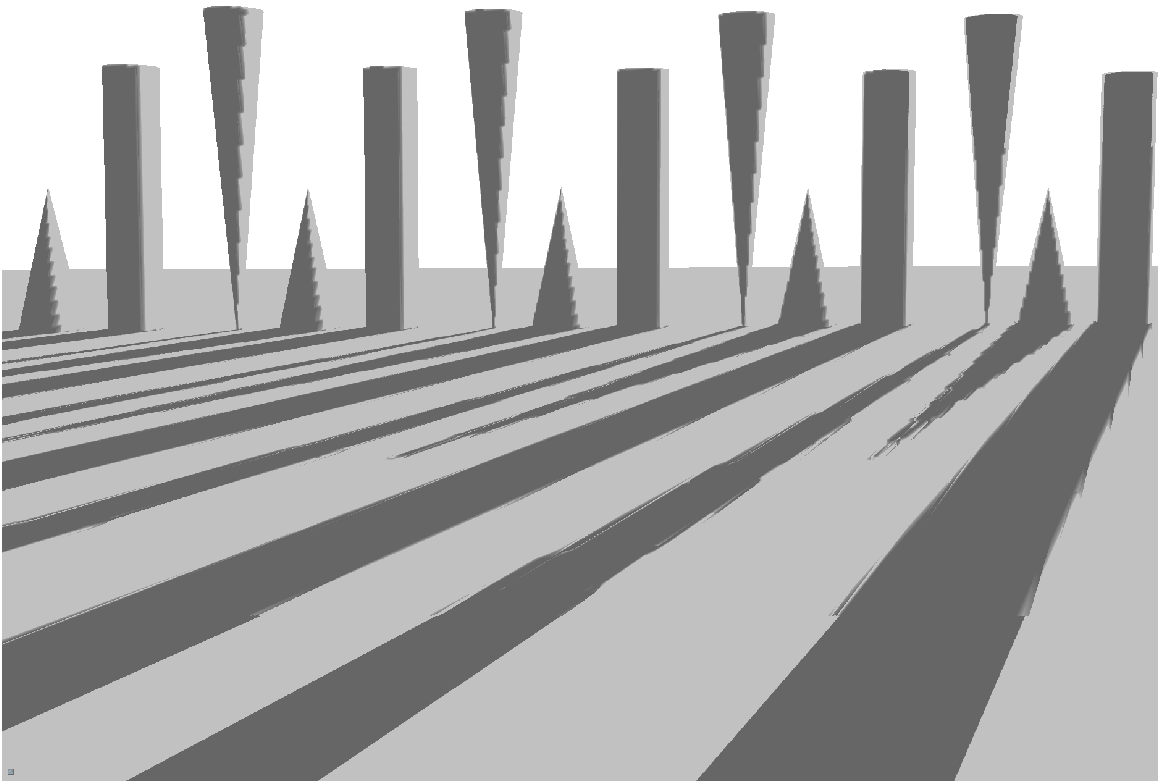
\includegraphics[width=0.48\textwidth]{pcsm_1b.pdf}\label{Teaser:b}
\caption{\small Shadows from a moving directional light rendered using two shadow map cascades. 
The first (near) cascade is updated every frame, and the second (far) cascade is cached 
and invalidated infrequently. The left image shows a mismatch 
between the cascades since the cached cascade is rendered
with a light direction that was captured many frames ago. Parallax correction fixes this divergence as shown
on the right image.}
\label{Fig:Teaser}
\end{figure}

However, caching is problematic when the shadow casting light is dynamic,
e.g. in a game with dynamic day-night cycle where the sun or moon is constantly 
moving across the sky, thus making cached data inconsistent with the current light
state. One has to either invalidate
the cache often to keep the divergence small, which makes caching a less
efficient optimization, or treat cached shadows as a very rough approximation of 
actual shadows because the error is too apparent when viewed up close.

In this paper, we describe a parallax correction algorithm for rendering 
sweeping shadows from a dynamic light source using a static shadow map. 
The use of parallax correction in \textit{Far Cry 5} enabled a fairly seamless
transition between dynamic shadows rendered with two different techniques:
near shadows with \textit{cascaded shadow maps} (CSM) updated every frame, and far shadows 
with \textit{adaptive shadow maps} (ASM) covering 500 meters range and updated every 2500 frames.
As a result, we are using relatively expensive CSM for rendering shadows within
only 30 meters from the player's camera, which is quite a short range for an open world game.

\section{Parallax Correction Algorithm}

When rendering images of a static scene from different viewpoints, one 
can reproject pixels seen from one viewpoint to another provided that 
the image depth buffer is available and we know all required camera transforms,
e.g.~\cite{Reprojection}. It is straightforward to apply this approach to shadow
maps: given a shadow map rendered with a shadow camera built for light direction
$L_0$, one can reconstruct world space positions of all shadow map texels, and
then render the resulting set of points (as a point cloud or a mesh) into a shadow
map for a different light direction $L_1$. It's possible to employ a more 
sophisticated method of interpolation~\cite{Reprojection2}.
Unfortunately, these reprojection procedures are not very practical 
since they operate with the entire shadow map, which is often a
high-resolution image. Processing a lot of texels may be computationally expensive
even with relatively simple shaders. Moreover, doing reprojection
over a set of shadow maps arranged via some spatial subdivision scheme, such as cascaded shadow 
maps, isn't straightforward for the border texels, which might end up in 
a different cascade when rendered with a new light camera. Here
we attempt to approximate the reprojection for a set of pixels on screen instead 
of warping the entire shadow map.

\begin{figure}[t]
\subfloat[The shadow map is rendered for a light direction $L_0$. The point $P_{occ}$ 
is starting to occlude $P_1$ rather than $P_0$ when the light changes 
its direction from $L_0$ to $L_1$. Our idea is to sample shadows at $P_0$ using
the shadow map computed for light direction $L_0$, and take the resulting shadow factor
for shadow intensity at $P_1$.\label{PCSM:a}]
{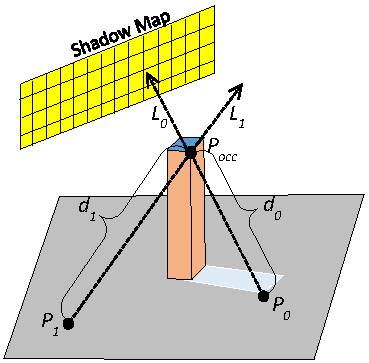
\includegraphics[width=0.48\textwidth]{pcsm_2a.pdf}}\hfill
\subfloat[We walk along the direction $D$ starting from $P_1$ in small increments,
sampling the shadow map at each point $S_i$ and accumulating occluder distance 
values. We stop after certain number of iterations. We compute the
average value of accumulated occluder distances, which gives us an 
approximation of $P_0$ via Eq. \ref{Eq:4}.\label{PCSM:b}]
{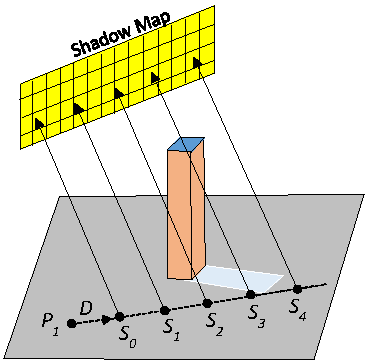
\includegraphics[width=0.48\textwidth]{pcsm_2b.pdf}}
\caption{\small Parallax correction algorithm.}
\label{Fig:PCSM}
\end{figure}

Assume we have a shadow map generated for a dynamic directional light with 
direction $L_0$. Consider a point $P_0$ in world space as illustrated in 
Fig.~\ref{PCSM:a}. We can reconstruct the world space position of its occluder 
$P_{occ}$ by computing the distance to occluder $d_0$ from the shadow map depth:
\begin{equation}\label{Eq:1}
P_{occ} = P_0 + d_0\;L_0.
\end{equation}
Suppose the light is moving, and its new direction is $L_1$. Let's project
$P_{occ}$ along the new direction $L_1$ to get a point $P_1$:
\begin{equation}\label{Eq:2}
P_1 = P_{occ} - d_1\;L_1.
\end{equation}
The practical meaning of (\ref{Eq:2}) is that we can compute shadows at 
$P_1$, i.e. $P_1$ will be in shadow for any $d_1 > 0$. So far we were following
this reprojection route: take a point $P_0$, reconstruct its occluder from 
a shadow map, and then use the reprojected occluder when shading the scene. However, 
we are really interested in doing these steps in the reverse order. For any 
given light direction $L_1$ and a point $P_1$, we want to find the corresponding
$P_0$, so that we can sample shadows at $P_0$ using the shadow map computed for 
light direction $L_0$ and then use the resulting shadow factor for shadow
intensity at $P_1$.

Our parallax correction algorithm can be briefly described as this: we want 
to get to $P_0$ from $P_1$. For this, we need two things: a good guess of the 
direction from $P_1$ to $P_0$ and a good guess of the length of the path from
$P_1$ to $P_0$. Let's elaborate how to obtain these values. Substituting 
(\ref{Eq:1}) into (\ref{Eq:2}), we get
\begin{equation}\label{Eq:3}
P_0 = P_1 + d_1\;L_1 - d_0\;L_0.
\end{equation}
We attempt to solve (\ref{Eq:3}) by assuming $d_1 = k\;d_0$, where $k$ is
a constant. We will discuss how we choose the value $k$ later in this section.
Here we only note that this assumption enforces a certain relation between 
$P_1$, $P_{occ}$, and $P_0$. This gets us
\begin{equation}\label{Eq:4}
P_0 = P_1 + d_0\;( k\;L_1 - L_0 ).
\end{equation}
Thus, if we want to compute shadows for light direction $L_1$ at an arbitrary
point $P_1$, we can use (\ref{Eq:4}) to find corresponding point $P_0$
provided that we can compute the distance to occluder $d_0$ and choose 
a reasonable value of $k$. 

\begin{figure}[t]
\subfloat[Occluder search with 5 iterations and $k = 1.5$. We are sampling
shadow map depths at each step to compute the distance from a point on the ray 
to its occluder, if there's any. \label{OccluderSearch:a}]
{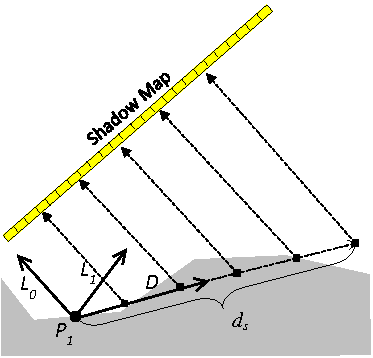
\includegraphics[width=0.48\textwidth]{pcsm_3a.pdf}}\hfill
\subfloat[Effect of parameter $k$ on search vector $D$. The value $k = 1.5$ 
would give incorrect results because some points on the search ray are located 
inside shadow casting geometry. \label{OccluderSearch:b}]
{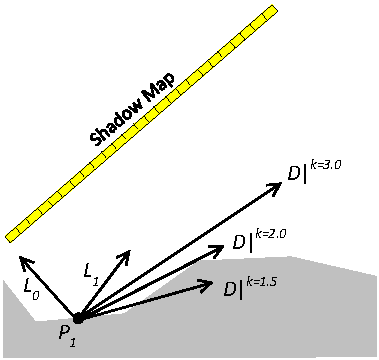
\includegraphics[width=0.48\textwidth]{pcsm_3b.pdf}}
\caption{\small Occluder search.}
\label{Fig:OccluderSearch}
\end{figure}

\bigskip
\textbf{Occluder search}. As follows from (\ref{Eq:4}), $P_0$ is located 
somewhere on the ray starting from $P_1$ in the direction 
\begin{equation}\label{Eq:5}
D = k\;L_1 - L_0.
\end{equation}
We search for an occluder by marching along this ray with a certain number
of iterations, computing occluder depth at each step, and then taking the average
for $d_0$. This process is illustrated in Fig.~\ref{PCSM:b} and 
Fig.~\ref{OccluderSearch:a}.

The search distance $d_s$ is a scene-dependent parameter that accounts for 
maximum displacement of the shadows due to the parallax we are expecting.
That is, we need a larger search distance for a scene with long shadows 
and tall shadow casting structures. Conversely, the search distance may 
be shorter for a scene with an overhead light and small shadow casters.
An increase in the difference between $L_0$ and $L_1$ also increases shadow
parallax and thus the search distance.

\bigskip
\textbf{Choosing the parameter $k$}. The point 
$P_0$ is located somewhere on the ray originating at $P_1$, with ray direction 
$D$ being controlled with the parameter $k$. Fig.~\ref{OccluderSearch:b} 
illustrates that changing the value of $k$ would result in different $D$, 
with values $k > 1$ corresponding to the point $P_0$ being closer to the occluder 
than $P_1$. Ideally, having $P_0$ on the surface of an object containing $P_1$ 
would give the most accurate shadows, but this is hardly possible in practice.
In our example $P_0$ will be either above the surface if we choose $k = 2$ 
or $k = 3$, or even below the surface if we choose $k = 1.5$.

The best value for $k$ depends on the scene. 
Consider a difficult situation when we want to compute parallax correction at
a point located on a concave surface. It's quite probable that the occluder search 
may be testing points under the surfaces of nearby objects as illustrated in 
Fig.~\ref{OccluderSearch:a}, thus interpreting surrounding geometry as an 
occluder.
Choosing a larger value for $k$ can help prevent these errors in concavities, as shown in 
Fig.~\ref{OccluderSearch:b}. However, a larger values of $k$ can cause the method 
to miss smaller occluders, thus producing inaccurate results. Due to this tradeoff, one needs
to pick the value of $k$ that produces the best results for a given scene.

We use the following empirical formula, where $k$ depends on 
the magnitude of the difference between light directions

\begin{equation}\label{Eq:6}
k = 1 + \| L_1 - L_0 \|.
\end{equation}

Finally, we can gather all the bits we have described so far into the sample
code given in Listing~\ref{List:Parallax}.

\lstset{language=C}
\begin{lstlisting}[float,caption={Example implementation of the parallax correction 
for a simple orthogonal shadow map.},label=List:Parallax]
uniform float3 L0; // shadow map light direction
uniform float3 L1; // current light direction
uniform float4x3 searchParams; // contains search distance, etc.
uniform float4x3 worldSpaceToShadowMap;

float CalcShadow( float3 P1 /* a point in world space */ )
{
#if ENABLE_PARALLAX_CORRECTION
  float k = 1.0 + length( L1 - L0 );
  float3 D = k * L1 + L0;

  // Occluder search    
  float3 S = P1;
  float3 dS = mul( float4( D, 1 ), searchParams );
  float sum = 0, cnt = 0;
  for( int i = 0; i < OCCLUDER_SEARCH_ITS; ++i ) {
    float3 Sp = mul( float4( S, 1 ), worldSpaceToShadowMap );
    float occDepth = SampleShadowMapDepthTexture( Sp.xy );
    if( occDepth < Sp.z ) {
      sum += Sp.z - occDepth;
      cnt += 1;
    }
    S += dS;
  }

  float d0 = cnt > 0 ? sum * rcp( cnt ) : 0;
  float3 P0 = P1 + d0 * D;
#else
  float3 P0 = P1;
#endif    
  // Compute shadow factor at P0
  float3 Pp = mul( float4( P0, 1 ), worldSpaceToShadowMap );
  return step( Pp.z, SampleShadowMapDepthTexture( Pp.xy ) );
}
\end{lstlisting}

\bigskip
\textbf{Implementation enhancements}. The accuracy of shadows created with parallax correction generally 
degrades as the angle between the current light direction and the original light direction increases.
It's possible to reduce the divergence 
and thus the visual deficiencies if we know the animation curve of the light $L(t)$,
where $L$ is the light direction and $t$ is time. Assume we want to update the shadow
map at regular time intervals with the time step $\Delta t$, i.e. if we first update
the shadow map at $t_0$, then the following updates will happen at $t_0 + n\;\Delta t$,
where $n$ is a positive integer. The best strategy when updating the shadow map at $t_0$
would be to take the light direction at halfway between directions $L(t_0)$ and 
$L(t_0 + \Delta t)$, or just taking $L(t_0 + \frac{\Delta t}{2})$
if the light's animation speed is constant. This minimizes angles between the light directions
used for shading and the direction of the shadow map. Even though  
lookahead sampling requires 
us to give the shadows subsystem access to the curve $L$ (thus making the implementation more complicated),
we found that the resulting improvement in quality is worth the effort. 

Another way to improve parallax-corrected shadows is adding a cross-fade 
when updating cached shadow maps to the most recent light state. We are assuming 
that two shadow map textures will be available at this point. It makes sense 
to render the updated shadow map into a separate texture because its rendering may take
several frames to complete (e.g. it takes more than 80 frames to update the cached shadow map 
in \textit{Far Cry 5}) and we still need to apply shadows to the scene while the new shadow map is 
only partially rendered, and thus it can't be used for shading. With both the old and new shadow
maps ready, we can perform a cross-fade between shadow factors sampled from these textures, which
is less visible than an immediate switch between the textures in a single frame.

\bigskip
\textbf{Algorithm limitations}. While the algorithm works well as long as the 
parameters $d_s$ and $k$ are chosen appropriately, a high variation in depth of
overlapping shadow casters results in incorrect parallax correction. It is
caused by the occluder search hitting the furthest occluder and computing parallax
correction using a biased occluder distance, which may distort shadows from closer
shadow casters overlapping with shadows from more distant ones, as shown in Fig.~\ref{Fig:FusionProblem}.
This is similar to the occluder fusion problem existing in some soft shadows algorithms, such as
\textit{percentage-closer soft shadows} (PCSS)~\cite{PCSS}.

\begin{figure}[t]
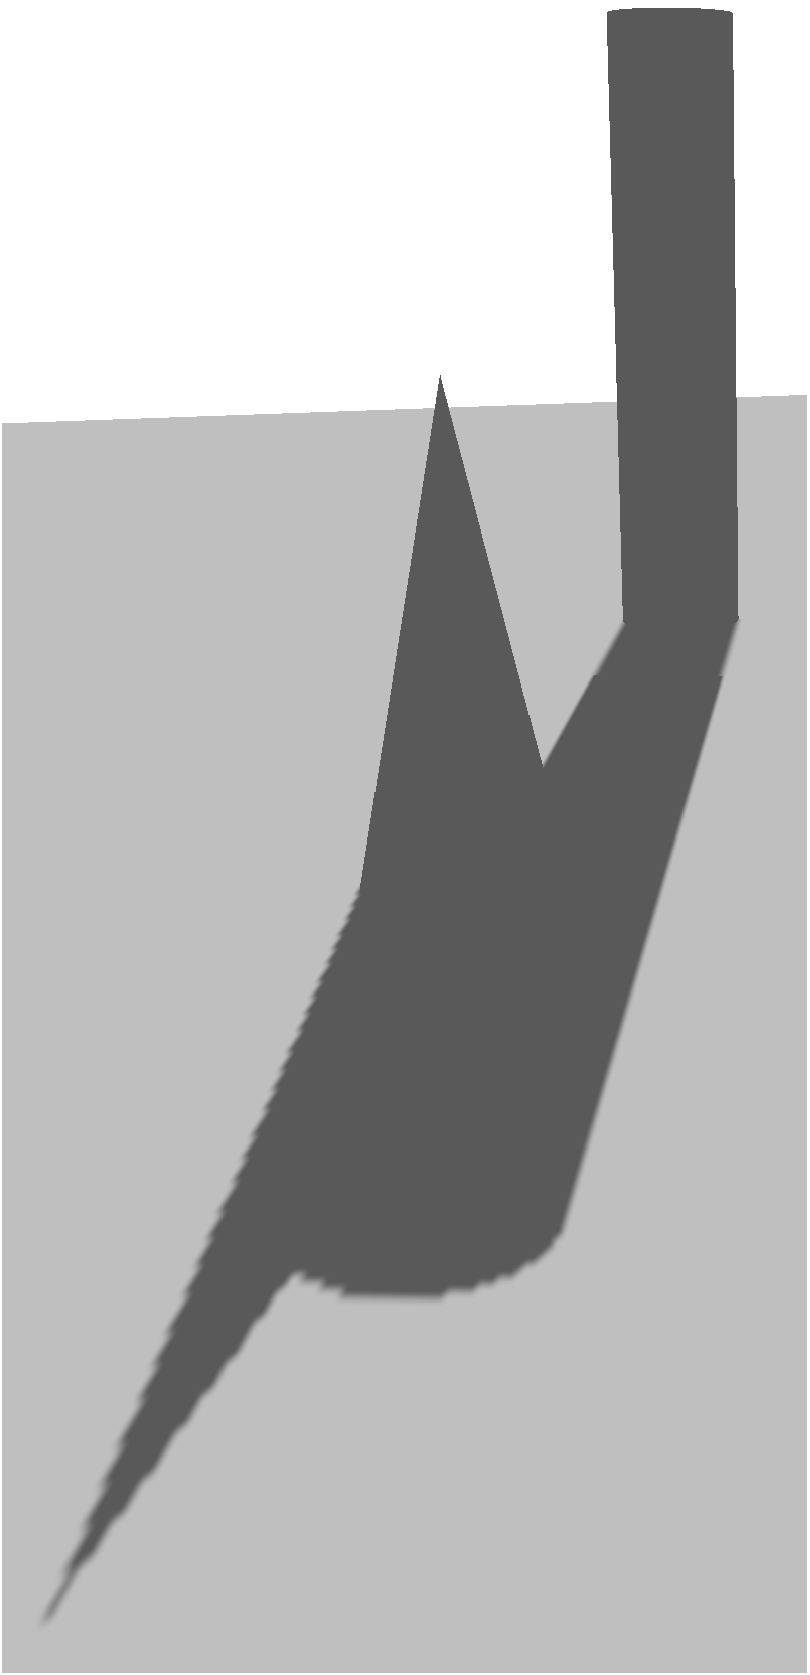
\includegraphics[width=0.24\textwidth]{pcsm_new_a.pdf}
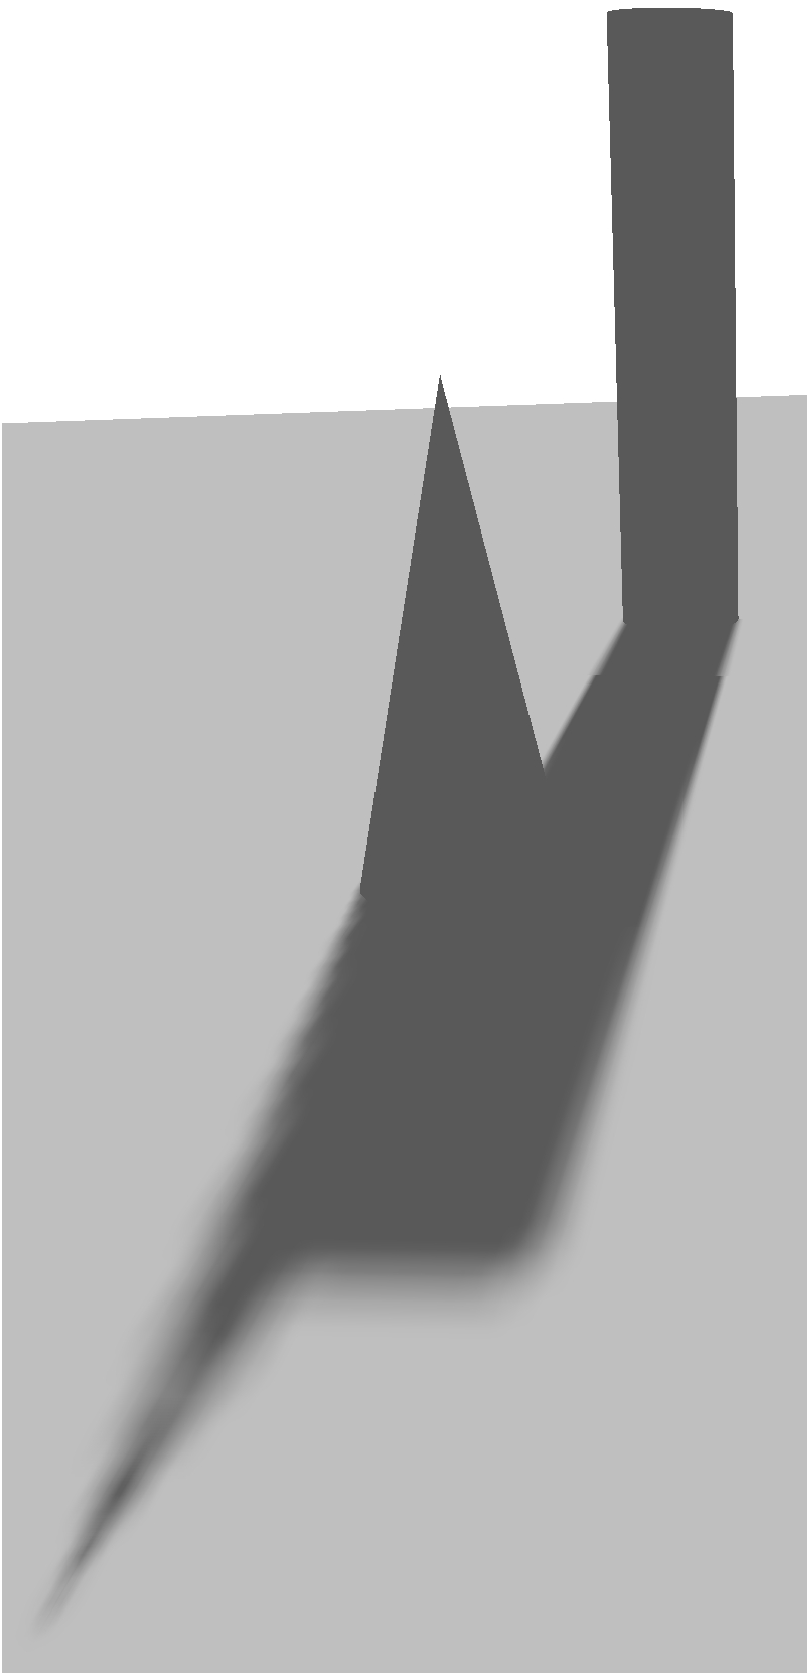
\includegraphics[width=0.24\textwidth]{pcsm_new_b.pdf}
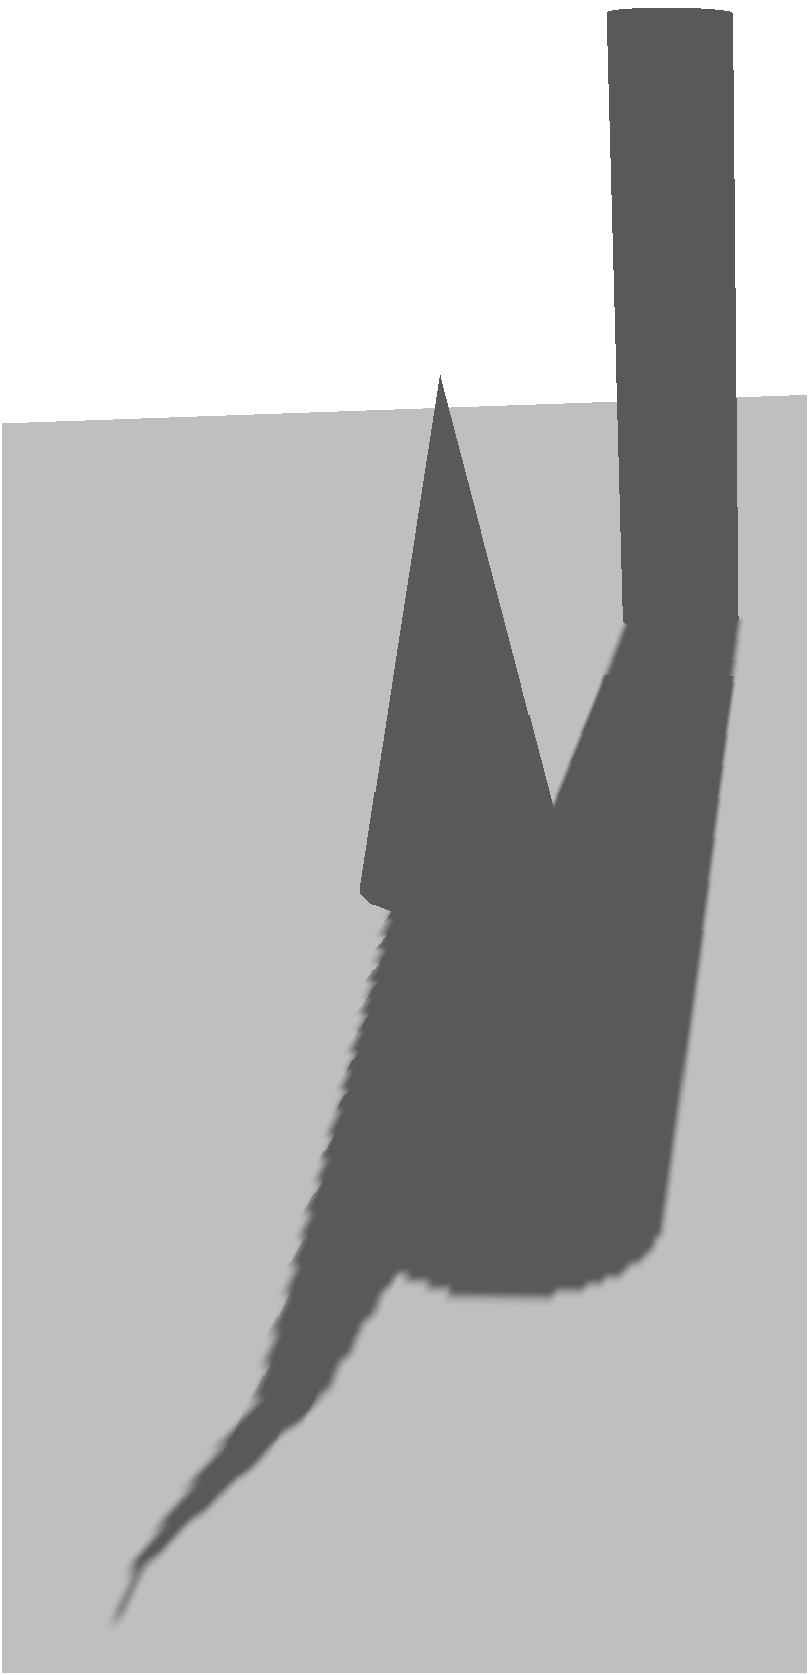
\includegraphics[width=0.24\textwidth]{pcsm_new_c.pdf}
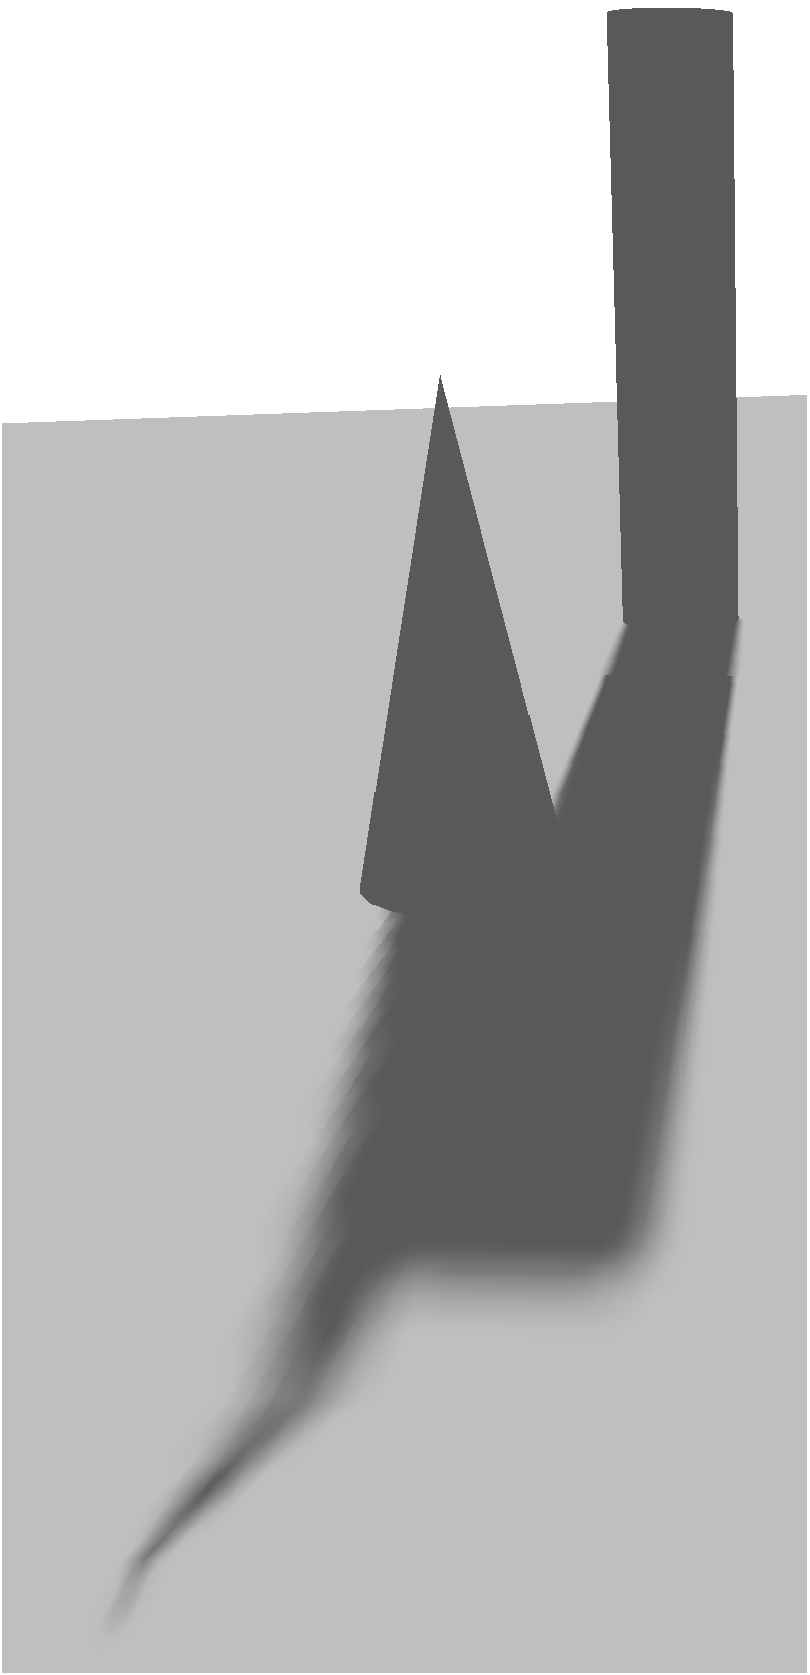
\includegraphics[width=0.24\textwidth]{pcsm_new_d.pdf}
\caption{\small Defects occuring with high depth variation of overlapping shadow casters. From left to right: a shadow from the cone is
overlapping with a shadow from the cylinder, which is much taller and further away from the camera;
PCSS estimator gives incorrect penumbra size resulting in a large penumbra near the cone base; our parallax correction algorithm also
produces incorrect results for the same reason (overestimation of the distance to occluder) resulting in shadows distortion; 
parallax-corrected shadows penumbra is incorrect too.}
\label{Fig:FusionProblem}
\end{figure}

\section{Applications of Parallax Correction}

Parallax correction may be applied to a number of algorithms that utilize 
shadow map caching. 
Generally, a static shadow-casting algorithm can be used to generate the initial shadow
map. Parallax correction can then be applied to adjust the map as lights move.
However, the caches need to be invalidated from time to time since 
parallax correction is an approximative technique.

\bigskip
\textbf{Cached cascaded shadow maps}. CSM
caching implies that not all cascades are updated within one frame. One way
to do that is skipping cascade updates for a certain small number of frames, either 
replacing cascade updates with another workload of similar complexity or 
updating distant cascades in a round-robin manner. The system keeps using 
matrices and shadow map textures cached from previous frames to apply shadows to
the current scene. We suppose that applying parallax correction in this scenario 
doesn't offer a lot of improvements since shadow maps are meant to be updated 
quite frequently (every other frame or so), thus small 
discrete changes in light direction aren't too noticeable.

The work \cite{CrytekRyse} employs a different approach to caching with a single shadow 
map containing only static objects replacing the last two cascades. Shadows
cover 1.4 km range, so the full update of this shadow map takes 10-15 ms 
distributed over many frames. In this scenario, parallax correction can reduce the visual 
discontinuity between the cascades that
is caused by the lengthy shadow map update process, similar to what is
demonstrated in Fig.~\ref{Fig:Teaser}. One should just update the static shadow map 
periodically rather than only in certain preset points in game levels.

\cite{CSMScrolling} utilizes a \textit{toroidal update} scheme, also found in other 
algorithms such as clipmaps~\cite{ToroidalUpdate}, to minimize the number of shadow casting objects 
rendered into cascades. Their main observation is that moving the player's camera only 
changes the cascade's frustum translation, but not its size or orientation, 
as long as the shadow casting light is static. Typically there's only a small difference 
between the current frustum and the frustum from the previous frame. Thus, 
contents of the shadow map would nearly be the same save for few 
small regions. One can perform a toroidal update reusing a large 
portion of the previously rendered shadow map, and only rendering objects 
falling into the parts near the shadow map border that were invisible previously. Parallax 
correction improves consistency between the cascades updated every frame 
and the cascades updated via toroidal update, thus allowing cached data to 
be reused for a longer period before the cached cascades need to be
rebuilt with a new light direction.

\begin{figure}[t]
\subfloat[ASM shadows from a mix of new and old tiles.\label{ASM:a}]
{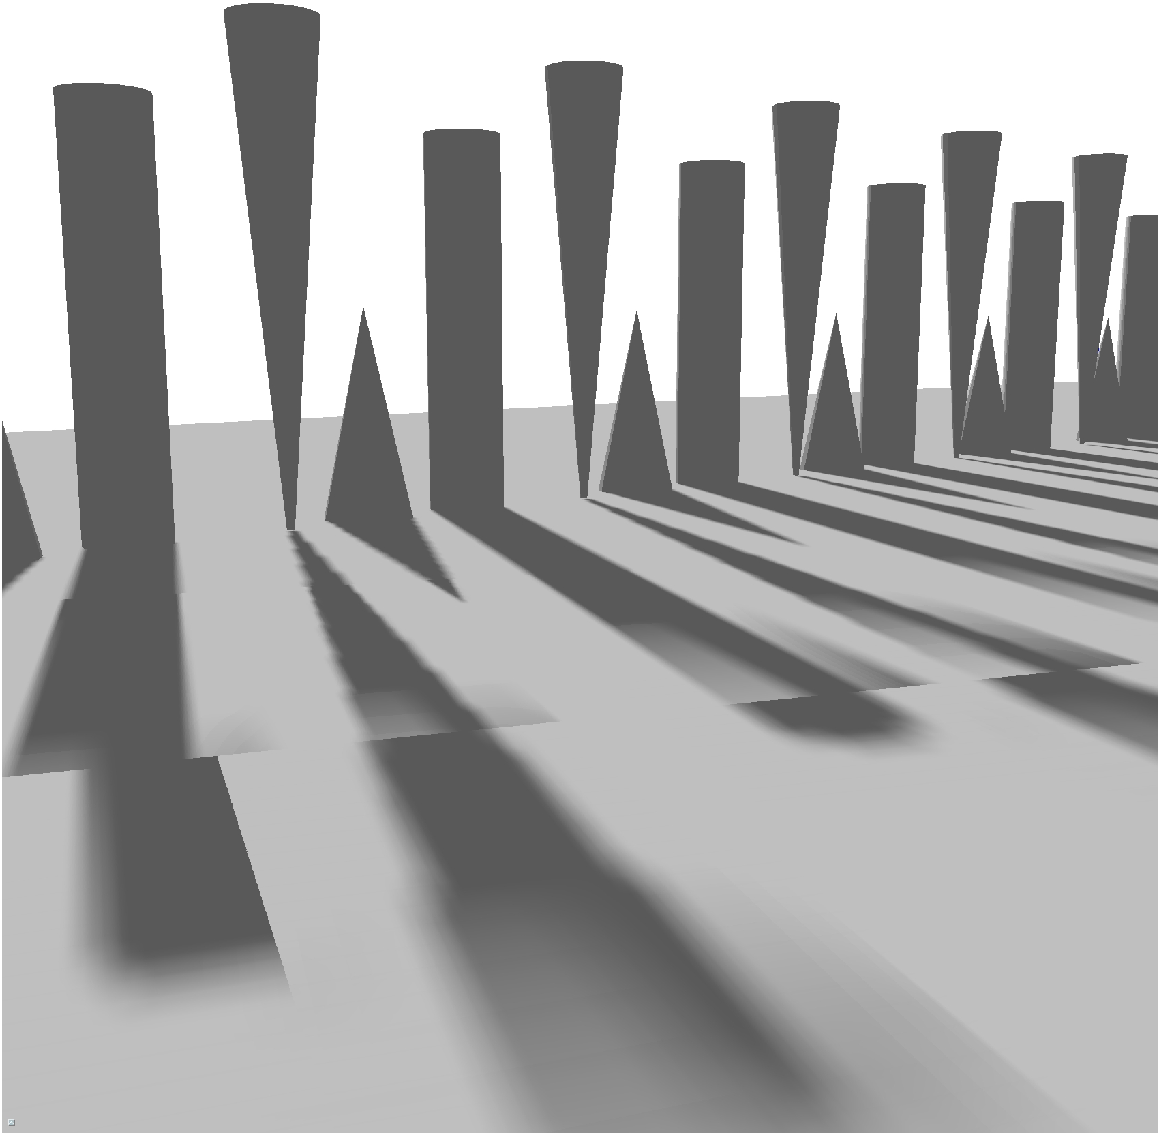
\includegraphics[width=0.48\textwidth]{pcsm_4a.pdf}}\hfill
\subfloat[The same set of tiles with parallax correction applied.\label{ASM:b}]
{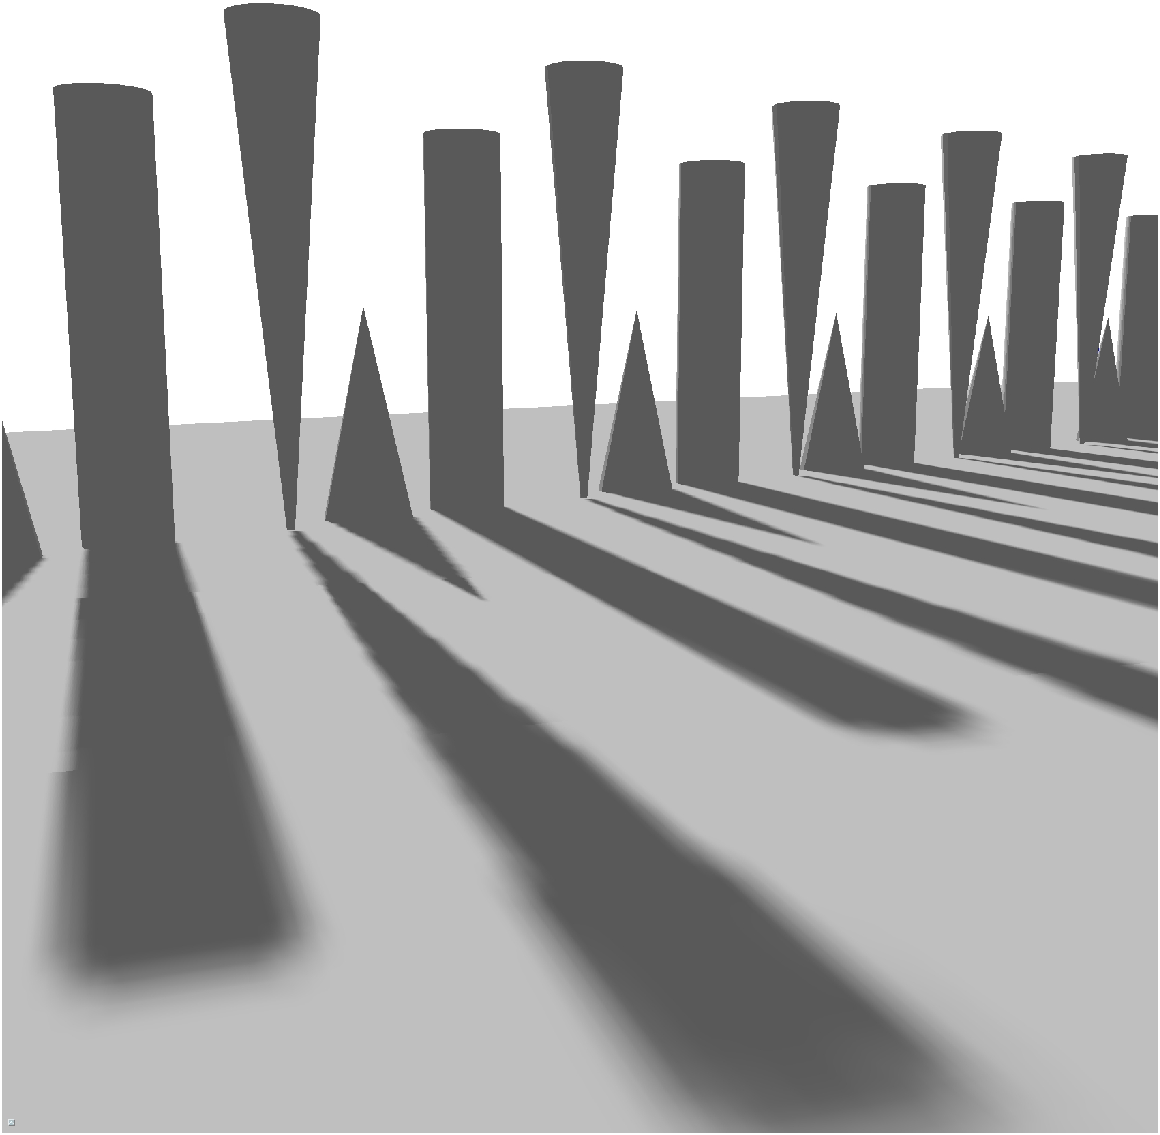
\includegraphics[width=0.48\textwidth]{pcsm_4b.pdf}}
\caption{\small Parallax correction not only enables smooth sweeping shadows 
with adaptive shadow maps algorithm, but also makes it possible to start 
evicting old tiles from the cache before the update is fully finished without 
having discontinuities visible in \protect\subref{ASM:a}.}
\label{Fig:ASM}
\end{figure}

\bigskip
\textbf{Adaptive shadow maps}. Shadow map caching is an essential part of 
the adaptive shadow maps algorithm, e.g.~\cite{ASM11}. It's possible to discretize 
light direction movements and build a separate hierarchy of tiles for each 
quantized light direction. Aside from possibly noticeable steps in the light 
directions, this also implies that we have to maintain two hierarchies whenever 
we want to update the shadow maps. One of the hierarchies is used for 
shading the current frame, and the other one is in the process of 
construction. Having two hierarchies at the same time means we need to 
double the size of the tile cache, and we also pay extra costs to render 
the tiles. Parallax correction addresses these issues.

We can start using the tiles rendered with the new light direction 
as they become available, rather than waiting until the full tile hierarchy
is ready. This way shadows are sampled from a mix of old and new tiles 
with the parallax correction ensuring shadow consistency as shown in 
Fig.~\ref{Fig:ASM}. Therefore, we can start discarding old tiles as the new tiles 
become available, thus reducing tile cache memory requirements and 
improving cache utilization.

\section{Results}

A major challenge in the development of \textit{Far Cry 5} was the addition
of new rendering techniques, such as screen-space reflections, that were not present 
in the engine previously. The existing subsystems 
had to become faster to accommodate for the new tech, thus the shadow rendering budget was 
reduced from 6 ms to 4.5 ms. The \textit{Far Cry} series has a long history of using cached shadow maps
\cite{ShadowsInGames}. However, cached shadows were always treated as a low-quality
solution for the objects further away from the player's camera, hence cascaded shadow maps
used to cover quite a large viewing distance. Adding parallax correction and 
improving cached shadow map filtering quality allowed having cached
shadows closer to the camera, thus reducing the range covered by CSM from 80 to 
30 meters. Table~\ref{Table:PerfCSM} shows examples of the resulting performance improvements.

\begin{table}[h]
\centering
\begin{tabular}{|c|c|c|c|c|}
\hline
\multicolumn{1}{ |c| }{\multirow{2}{*}{Test} } &
\multicolumn{2}{ |c| }{Number of objects in CSM} &
\multicolumn{2}{ |c| }{CSM GPU render time, ms} \\
\cline{2-5}
\multicolumn{1}{ |c| }{} & 80 meters & 30 meters & 80 meters & 30 meters\\
\hline
a & 310 & 104 & 3.8 & 2.3\\
\hline
b & 132 & 68 & 3.9 & 2.8\\
\hline
\end{tabular}
\caption{\small Reducing the range of cascaded shadow maps was a large 
win performance-wise. \textit{Far Cry 4} used CSM with three cascades covering 80 meters
range from the player's camera. We have reduced the range of three cascades down to 30 
meters in \textit{Far Cry 5}, since parallax-corrected adaptive shadow maps are good enough
to be used at ranges closer than 80 meters. A great side effect of this range
reduction was the increase of CSM texel density around the player.}
\label{Table:PerfCSM}
\end{table}

We are using adaptive shadow maps for shadows covering the range from 30 to 
500 meters from the camera. A typical cost of rendering a single ASM tile is around 0.5 ms on
the GPU and up to 1.5 ms on the CPU on PS4. An ASM light direction update is triggered every 1--2
minutes of normal gameplay time, so we're avoiding the update costs in the vast majority of
frames. Our implementation of the parallax correction is relatively lightweight, with 
the typical GPU cost being 40-70 $\mu s$ on PS4. We are performing the occluder search with 7 steps 
over a low-res downsampled depth map generated using a min-depth
kernel over the shadow map (see \textit{depth extent map} in \cite{ASM11}), which
improves search accuracy while keeping the number of iterations low.

\begin{figure}[t]
\centering
\subfloat[A mismatch between long-range and dynamic shadows due to a slow update of 
cached long-range shadows.\label{FC5:a}]
{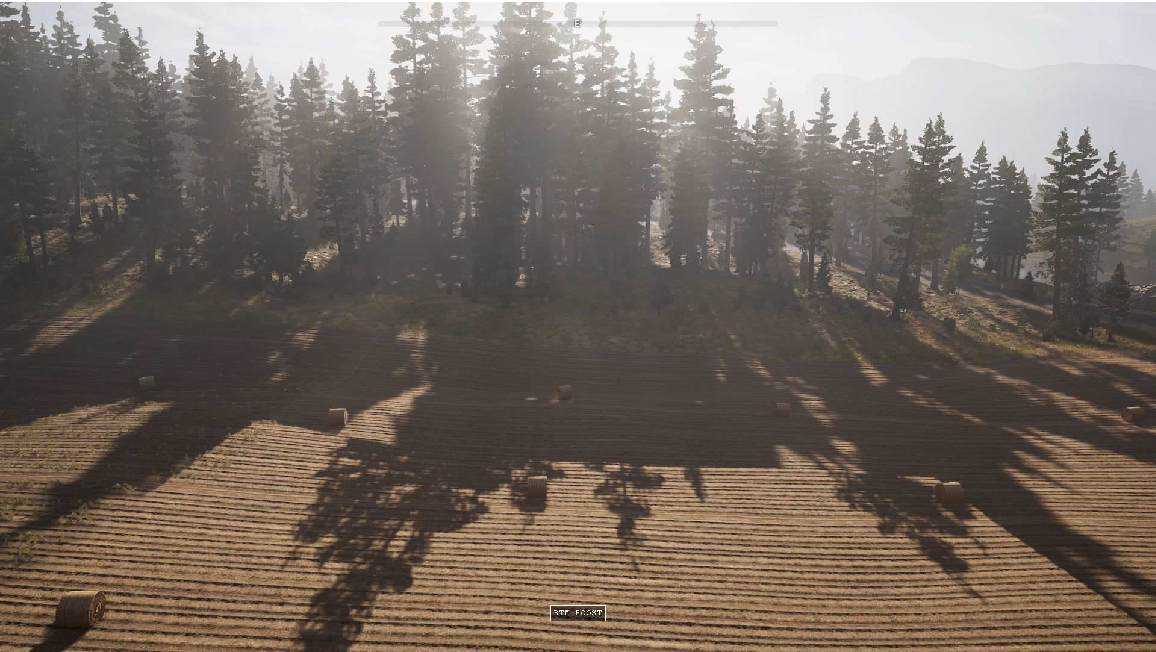
\includegraphics[width=0.9\textwidth]{pcsm_5a.pdf}}\\
\subfloat[Parallax correction fixes the mismatch so that the long-range shadows are
perceived as a level of details of dynamic shadows rather than something unrelated.\label{FC5:b}]
{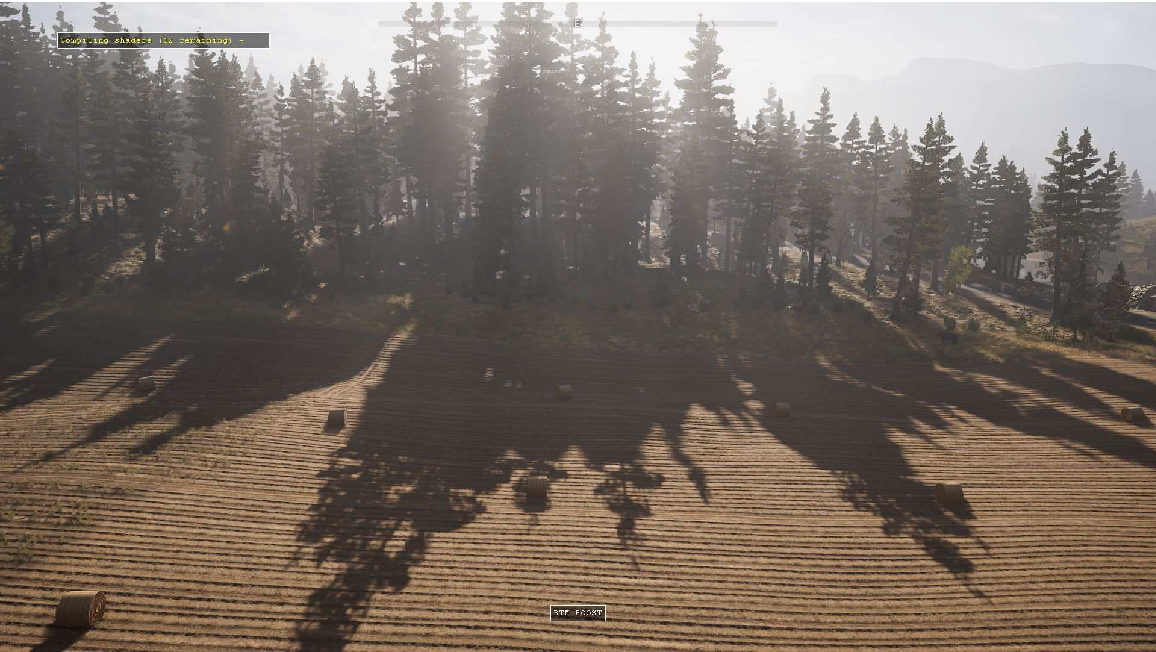
\includegraphics[width=0.9\textwidth]{pcsm_5b.pdf}}
\caption{\small Parallax correction improves the transition between cascaded shadow maps 
at the foreground and adaptive shadow maps at the background in \textit{Far Cry 5}.}
\label{Fig:FC5}
\end{figure}

The importance of consistency between cached and dynamic shadows is clearer 
in motion than on static screenshots such as Fig.~\ref{Fig:FC5}. Our very infrequently
updated cached shadows without parallax correction often resulted into lighting being completely 
different when transitioning between dynamic and cached shadow maps. In motion this change between
the two types of shadows was perceived as a cross-fade between unrelated images 
rather than a change in a shadow's details. See this book's online sample code for a demonstration of
parallax correction in motion.

\bibliographystyle{akpbib}
\bibliography{Turchyn}

%---END AUTHOR EDIT---

%*******************************************************************************
% Back Matter
%   Back matter begins with the bibliography.  We strongly recommend using a
%   .bib file.  You are welcome to use another bibliography style instead of our
%   in-house style.  For final production, the generated file can be renamed to
%   bibliography.tex. This file can be edited as needed, usually to fix breaks.
%
%   The index follows.  The index is generated using \makeindex (see above).
%   Use \printindex to display the index.
%
%*******************************************************************************
\backmatter
 \renewcommand{\chaptermark}[1]{\markboth{#1}{#1}}

\raggedright
\printindex

\end{document}
